{\em Note that in this chapter, the optimal method for selecting $F_{inf}$ has not necessarily been used to produce all plots or all conclusions. That is a subject for later exploration and refinement.}

In the last chapter, $\psi_l$ was defined as the sum over $m$ within a specific l-mode. To obtain the total self-force, it is necessary to sum all of these l-modes, for every time, using the value of $F_{inf}$ selected for that mode. Naively, one might sum only those modes for which there is data-- only up to the maximum l-mode computed in the simulation. However, it is possible to do a fit to a functional form found in Reference~\cite{heffernan_ottewil_wardell_modesum_basisForCode} and use the analytic sum of that functional form to add the contribution from $l_{max}+1$ to infinity to the results computed from the simulation. The dependence of the m-summed self-force for a given mode on $l$, for large $l$, is shown below, modified to omit terms that are rescaled to zero by the definition of the effective source in~\cite{wardell_vega_thornburg_diener}.
\begin{eqnarray}
  F_r(l,t)=&\frac{A(t)}{(2l-1)(21+3)}+\frac{B(t)}{(2l-3)(2l-1)(2l+3)(2l+5)}\nonumber \\
  &+\frac{C(t)}{(2l-5)(2l-3)(2l-1)(2l+3)(2l+5)(2l+7)}+\ldots
  \label{lmodefitsum}
\end{eqnarray}
Here $A(t)$, $B(t)$, and $C(t)$ are constants with respect to l determined by a least squares fit. Least squares fits minimize the sum of the squared differences between the function and the data in the $y$ direction, over all values of $x_i$. For fit parameters $A$, $B$, and $C$, and $l_{max}=n-1$, the portion of the total radial self-force contributed by the l-modes extrapolated to infinity after the end of the known data is given by
\begin{eqnarray}
  \sum_n^{\infty} F_r(l) = &\frac{An}{4n^2-1}+\frac{Bn}{3(9-40n^2+16n^4)}\nonumber\\
  &\frac{Cn}{5(2n-5)(2n-3)(2n-1)(2n+1)(2n+3)(2n+5)}+\ldots
\end{eqnarray}
Although Peter Diener's Fortran code implements this sum, I have analyzed it in an independent way to establish choices of $l_{min}$ and $l_{max}$ and to establish best choice DG orders for the code. In my computations, I have terminated the ``end of the known data'' at the end of the fit region, on the theory that I am simulating having more or fewer total l-modes available to me by including more or fewer l-modes in my fit.

\section{Fitting techniques and choice of starting mode}
\label{fitting}
A good fit should not have a systematic deviation to one side of the data. Such systematic deviations are often introduced in power-law fits in experimental data because the error stays about the same as the value decreases. Thus, constant errors are used in the fit, and data with a weak signal is given less importance.

However, it is difficult to apply this expectation to data in the truncation error regime of data generated from a numerical simulation. There are two differences. One is that the error is biased. While a good fit should still pass through the middle of the data in some sense, the truncation error may result in systematic deviations of the functional form of the self-force with l-mode. We believe we have corrected this to first order using a Richardson extrapolation, but higher order deviations may remain.

Secondly, the second order error is not necessarily expected to remain constant with l-mode. Ideally one would do a second order Richardson extrapolation to take the second order error into account and compute the truncation error, but our data is too sparse in starting orders with solutions. Instead, I assume the error is random and scales in two different specified manners, $\sigma^{-1}$ and $\sigma^{-2}$. This is neither the classical manner of computing the roundoff noise nor the truncation noise; however, it should improve a least squares fit and therefore improve stability and accuracy in the simulation.  

In these fits, I minimize the classic $\chi^2$ with weights, as follows
\begin{equation}
\chi^2=\sum_i \frac{(y_i-f(x_i))^2}{\sigma_i^2}
\end{equation}
Since the $\sigma_i$ weights do not represent proper statistical uncertainties, the normalization of the weights is unimportant, unless they are used to interpret the ``goodness'' of a fit in terms of a reduced chi-squared. Since the error behaves in an unknown, possibly highly correlated, deterministic, manner, cation is warranted in doing so. I have examined weights that are constant (effectively no weight), that  scale as $l^{-2}$, and that scale as $l^{-1}$. The first is motivated by standard fitting techniques and is the default solution, while the second is motivated by the nature of the first order scaling behavior of the function to which we fit the l-modes, and the third is motivated by the desire to find something that behaves well in both the truncation error and roundoff error regimes. Figure~\ref{sigmafit} shows the functional form of the l-mode fit with three different choices of weights. Figures~\ref{8badfit} and~\ref{14goodfit} show that for all choices of weight scaling, a starting l-mode of 14 is a reasonably good fit, while significantly lower starting modes are a bad fit for three terms in the l-mode fit expansion. These figures also show that the choice of sigma can make a small difference in the goodness of the fit at high l-mode, which is important for extrapolation to infinite l-mode. However, Figure~\ref{scatterfig} shows that for a range of $l_{min}$ versus $l_{max}$, the variation in the total radial self force due to variation over start and stop range in the fit is small compared to the variation between between $l^{-2}$ scaling and constant scaling (circles and triangles). 

\begin{figure}
  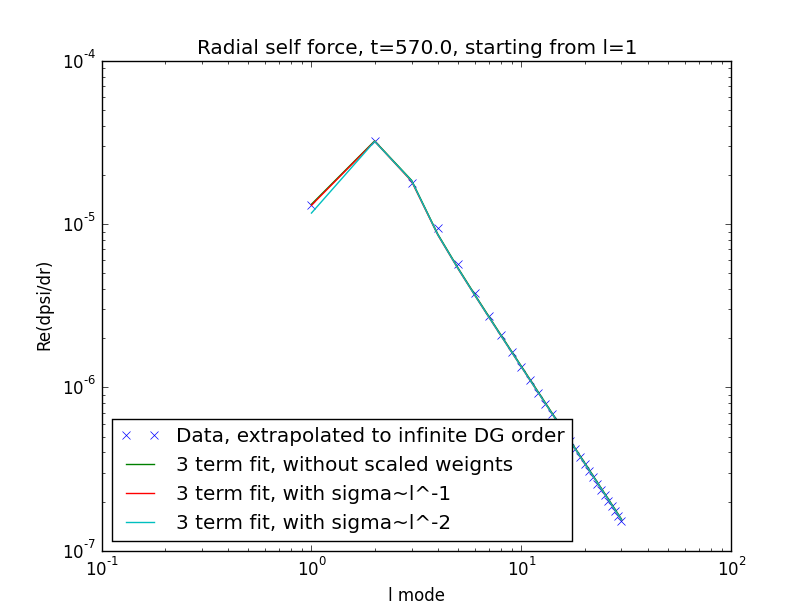
\includegraphics{fiterrscalecorrect3term570l1}
  \caption{The l-mode convergence behavior and three different fits to it using three terms in the l-mode fit sum of Equation~\ref{lmodefitsum}. The three different fits represent different choices of weights in the least squares fit.}
\label{sigmafit}
\end{figure}

\begin{figure}
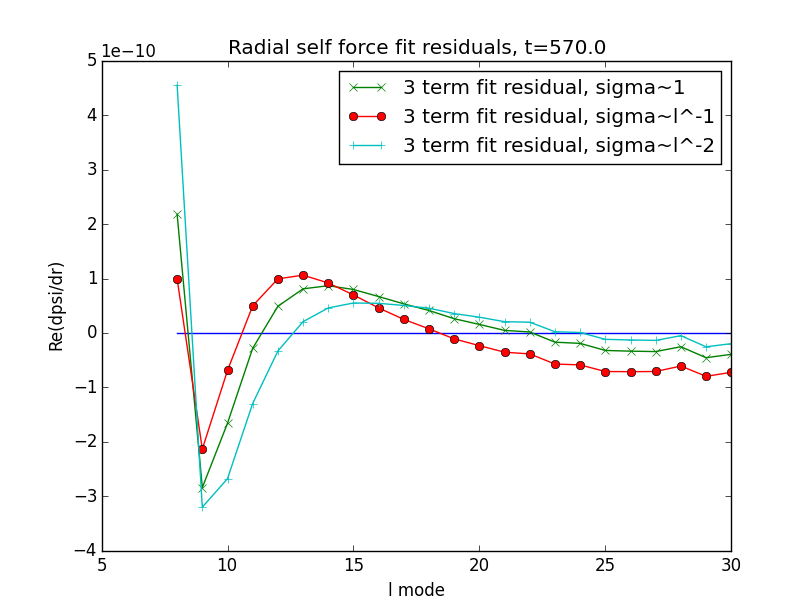
\includegraphics{fitresiduals3terms570l8}
\caption{Fit residuals for three different least squares weight scalings starting from $l_{min}=8$ to $l_{max}=30$. Notice that this is a bad fit, due to the strong correlated skews to either side of the axis.}
\label{8badfit}
\end{figure}

\begin{figure}
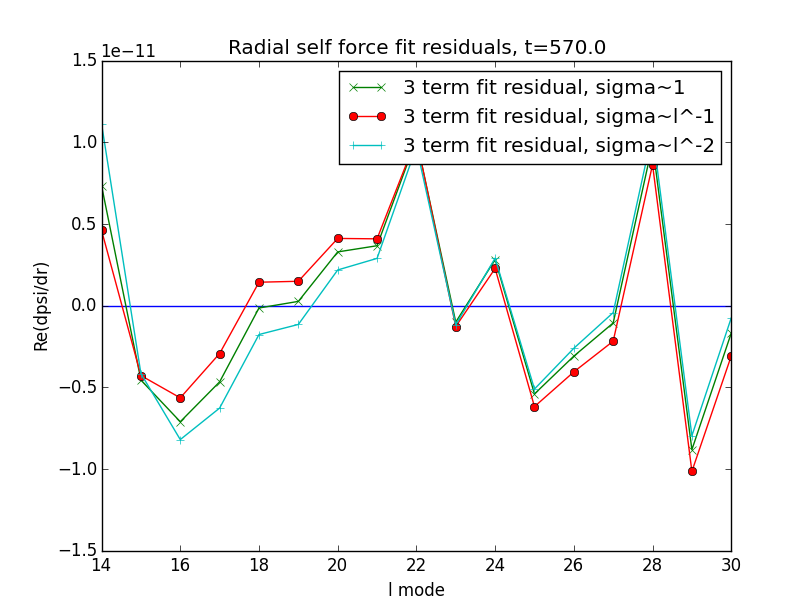
\includegraphics{fitresidulas3terms570l14}
\caption{Fit residuals for three different least squares weight scalings starting from $l_{min}=14$. This is a much better fit than $l_{min}=8$ to $l_{max}=30$ both due to the smaller correlated deviations from zero and due to the smaller amplitude of the residual.}
\label{14goodfit}
\end{figure}

\begin{figure}
  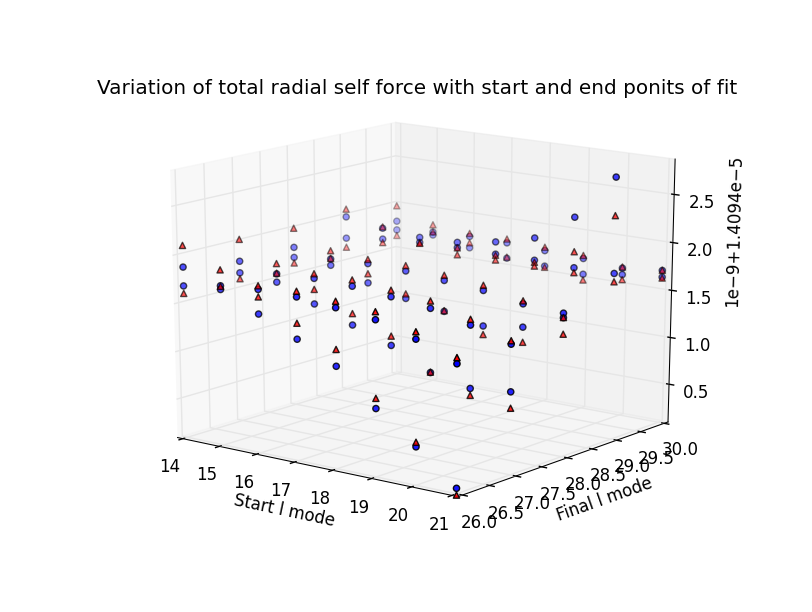
\includegraphics{3Dscatterwithwithoutsigmalminlmax}
  \caption{The difference between the triangles and the circles shows that the difference in the total radial self force between the presence of a $\sigma\sim l^{-2}$ weight and no weight is unimportant compared to the difference in the total radial self force between various start and end points of the l-mode fit.}
  \label{scatterfig}
\end{figure}

\section{Roundoff noise and choice of end mode}

In Figure~\ref{surface234big} roundoff noise is evident at higher $l_{max}$ choices, where $l_{min}$ is the minimum l-mode included in the fit and $l_{max}$ is the maximum l-mode included in the fit. This is most true of times near apastron. Note that there is not a large difference between two and three terms, and that four terms is less smooth a surface, suggesting that it is more subject to variations in the fit due to a poor fit at high l. The systematic deviations in the plot are correlated because all regions to the right of mode 27 include mode 27 in the fit, for example. The upsurge at high l is most readily attributed to roundoff noise. In Figure~\ref{surface234small}, a smaller region of $l_{min}$ versus $l_{max}$ space has been chosen to form the surface plot where roundoff noise is excluded. Three terms is preferred due to its stability within this region.

\begin{figure}
  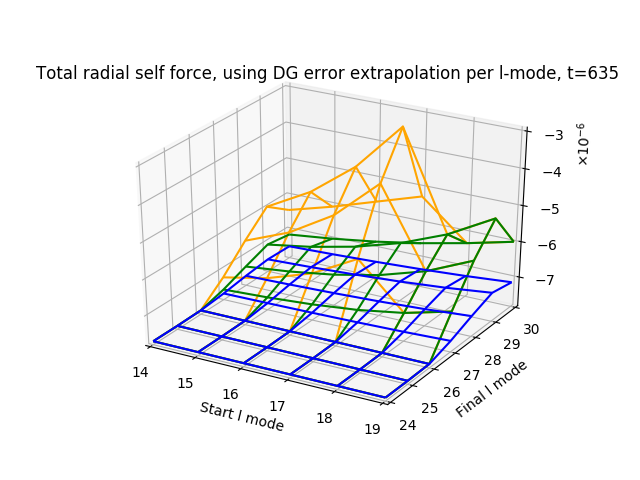
\includegraphics{bestfinflminlmax234terms635fullrange_perihelion}
  \caption{A surface plot of $F_{inf}$ generated using the median method, t=635, 2, 3, and 4 term fits over a broad range of $l_{min}$ and $l_{max}$ values. Note the roundoff noise at high $l_{max}$ that creates an upsurge in the surface. This is at apastron, where the roundoff noise effect is strongest. 2 is blue, 3 is green, 4 is orange.}
  \label{surface234big}
\end{figure}

\begin{figure}
  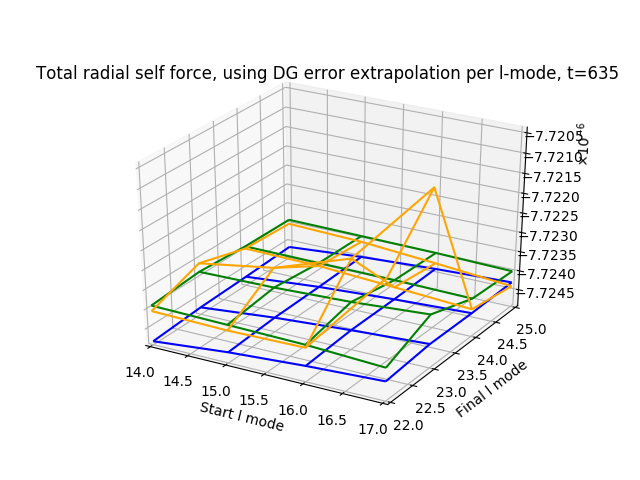
\includegraphics{bestfinflminlmax234termst635smallrange_perihelion}
  \caption{A surface plot of $F_{inf}$ generated using the median method. t=635, 2, 3, and 4 term fits over a small range of $l_{min}$ and $l_{max}$. This is near apastron where the roundoff noise is a dominant effect in the larger range of $l_{max}$.  No roundoff noise is evident in this range of $l_{min}$ and $l_{max}$ so it is a suitable range to consider at all times. 2 is blue, 3 is green, 4 is orange}
  \label{surface234small}
\end{figure}



\section{Results and errors}

Figure~\ref{totalselfforcevt} shows the evolution of the total self force over time. First it has been extrapolated to obtain $F_{inf}$ using the three-point DG order exponential convergence extrapolation technique, and the optimal starting order has been chosen. Then the modes computed in the simulation have been summed numerically from $l=0$ up to some $l_{max}$, and a fit from $l_{min}$ to $l_{max}$ has been used to extrapolate the sum to infinite $l$, to obtain the total radial self-force, at each time. 


\begin{figure}
  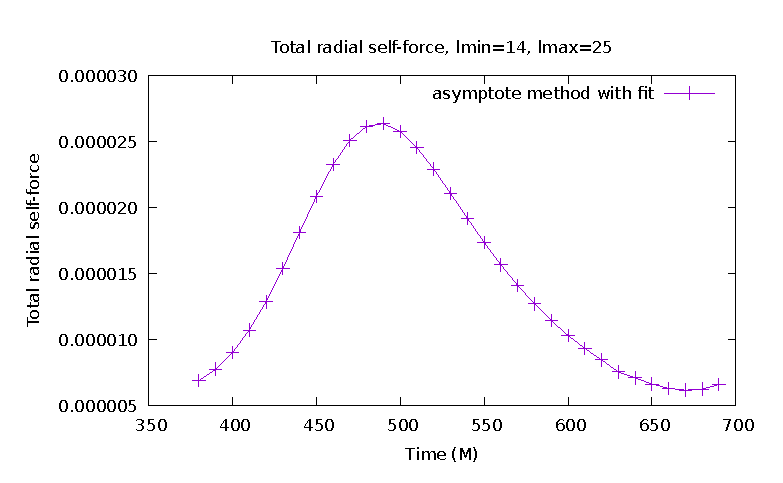
\includegraphics{totalselfforcevt2.eps}
  \caption{This is the total radial self force calculated using a l-mode sum including a contribution directly summing $F_{inf}$ from $l=0$ to $l=25$ and a contribution obtained using an analytic sum of the three term fit in Equation~\ref{lmodefitsum}. $F_{inf}$ is measured using the asymptote method defined in Chapter~\ref{finfchap} for selecting the best starting order}
\label{totalselfforcevt2}
\end{figure}


\subsection{Relative and absolute differences}

Figure~\ref{relErrSelfForceBigSmall} shows the relative difference between the total radial self force measured in two different ways. The self-force values in each surface plot shown in Figures~\ref{surface234big} and~\ref{surface234small} were averaged to obtain better estimates of the total radial self force as a function of time. This plot shows the relative difference. I use averages and standard deviations of correlated data with biased errors of data that is not fundamentally random, so they cannot be interpreted in the strictest of statistical senses; however, they should still provide some indication of the central value and spread of the data.

The relative difference introduced by the starting and end point of the fit is on the order of $10^{-4}$ based upon these averages. If individual modes were considered rather than averages, we might expect to see the resolution decrease by a factor of the square root of the ratio of the size of the two regions being averaged, due to the central limit theorem. That's a factor of $\sqrt{7\times 6}{4\times 4}=1.6$, which is not significant on the scale of four orders of magnitude. 


\begin{figure}
  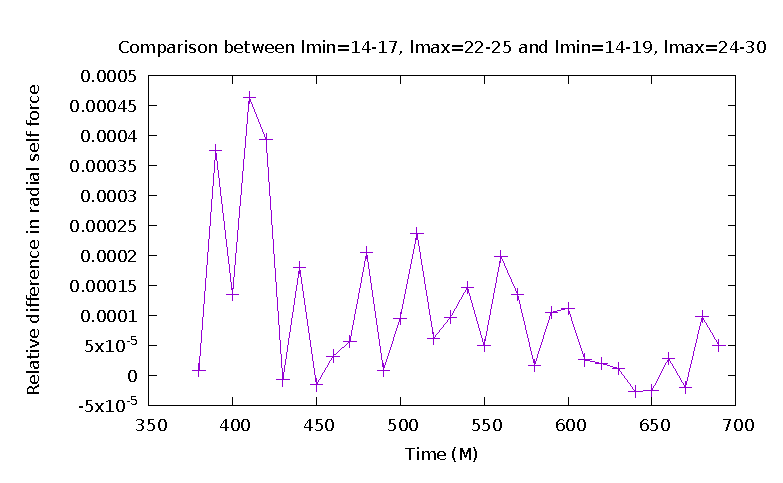
\includegraphics{relErrBigSmallRangeOverTime.eps}
  \caption{The relative difference between total self force determined by averaging large versus small ranges of total radial self-force $l_{min},l_{max}$ surfaces, as a function of time is at the $10^{-4}$ level.}
  \label{relErrSelfForceBigSmall}
\end{figure}


Figure~\ref{relErr23terms} shows the relative difference between using two and three terms in the fit to compute the total radial self force, as a function of time. Again, this is random, decreasing with time, and at the $10^{-4}$ level. 


\begin{figure}
  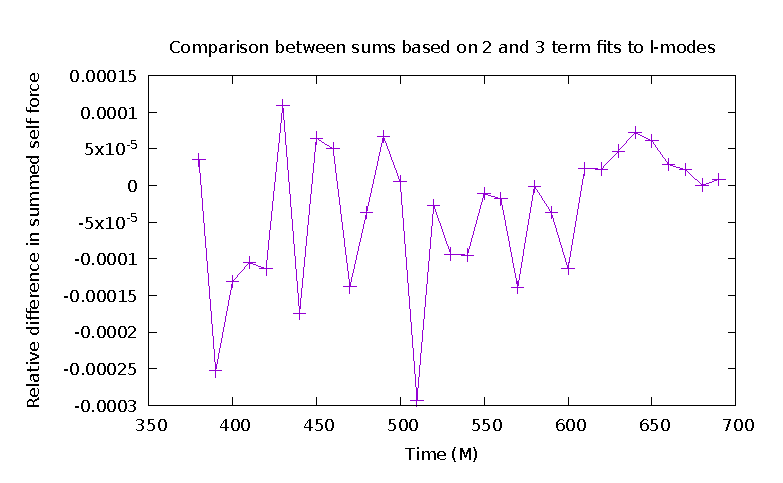
\includegraphics{relativeError23termSelfForce.eps}
  \caption{The relative error of the total radial self-force, comparing two to three terms in the l-mode fit.}
  \label{relErr23terms}
\end{figure}

The error due to the choice of the number of terms in the fit is comparable to the error due to the choice of start and end modes and the error due to our inability to use a first order Richardson extrapolation in real time. These errors are all at the level of a relative error of $10^{-4}$. The error due to the choice of fit method, visible from the offset between the triangles and circles, corresponding to the use of weights and no weights, can be seen in Figure~\ref{scatterfig} and is subdominant to the error introduced by the choice of $l_{min}$ and $l_{max}$ by at least an order of magnitude. 




\subsection{Fractional errors}


I obtain the fractional error, within a given method for choosing the best self force, by dividing the standard deviation of the total self-force, over a range of $l_{min}$ and $l_{max}$ by the average. This is shown for median and fit methods in Figures~\ref{medfracerr} and~\ref{fitfracerr}, respectively. The two methods are clearly not consistent in detail of their evolution, though they give roughly the same order of magnitude averaged over time. The absolute error is the standard deviation itself. The absolute error, as a function of time, compared to the self-force itself, is shown in Figure~\ref{twopeaks}. The two peaks do not obviously match periastron, apastron, or any specific phase of the orbit. {\em There is further work to be done here, specifically, I would like to redo this with the asymptote method.}


\begin{figure}
  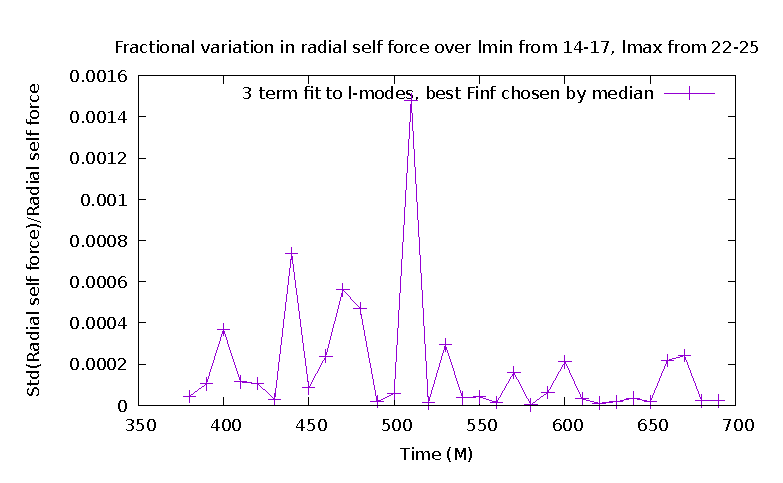
\includegraphics{fractionalErrorSelfForceOverTime3termMedian}
  \caption{Fractional error in total radial self force, with average and standard deviation calculated over the surface shown in Figure~\ref{surface234small}. Fractional error is defined as standard deviation divided by average. This figure is for 3 terms in the fit, using the median method. Fractional error is at the level of $10^{-3}$. $F_{inf}$ was determined using the median method to determine $F_{inf}$.}
  \label{medfracerr}
\end{figure}

\begin{figure}
  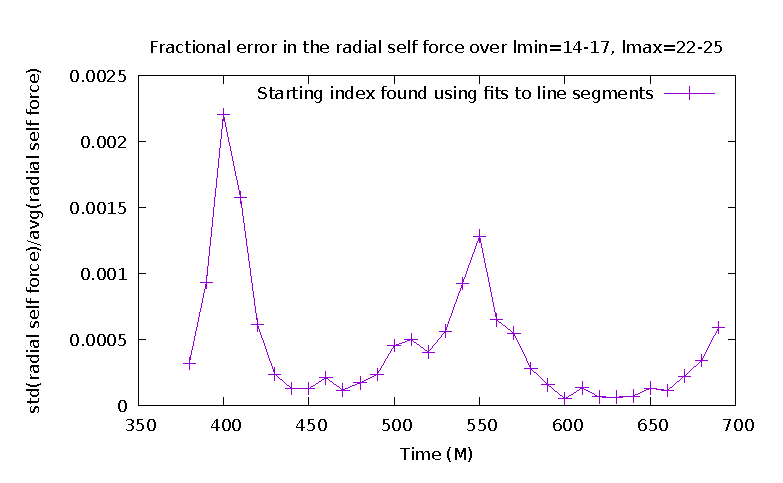
\includegraphics{fractionalErrorOverTimeFits}
  \caption{Fractional error in the total radial self force, with average and standard deviation calculated over the surface shown in Figure~\ref{surface234small}. Fractional error is defined as standard deviation divided by average. This figure is for 3 terms in the fit, using the fit method to determine $F_{inf}$. Fractional error is at the level of $10^{-3}$. $F_inf$ was determined using the fit method.}
  \label{fitfracerr}
\end{figure}


\begin{figure}
  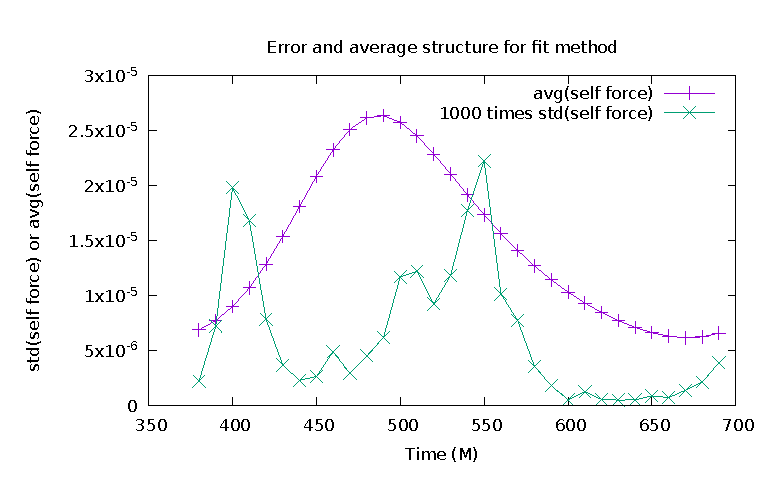
\includegraphics{structErrFitMethod}
  \caption{The structure of the standard deviation of Figure~\ref{surface234small} in comparison to the evolution in time. This is for the fit method for determining $F_{inf}$.}
  \label{twopeaks}
\end{figure}

Relative error compares one model to a different model. Fractional error compares the spread of parameters within a model. The order of magnitude larger fractional error in the l-mode start and end points than in the relative error measurement of these start and end points points to the importance of the corrections in the surface in Figure~\ref{surface234small}. To obtain an estimate of the error that is better than a two order of magnitude range from $10^{-3}$ to $10^{-4}$, it is necessary to perform either a proper second order Richardson extrapolation or a proper statistical study using covariances, hypothesis testing, and an as yet undiscovered method of handling biased estimators and unmodelled noise. 


\section{Best choice $l_{mins}$ and $l_{max}$'s and best choice DG orders}

$l_{min}$ can be as low as 14 and as high as 17, and $l_{max}$ can be as low as 22 and as high as 25 without encountering roundoff or truncation error. The errors are dominated by correlations in the choice of the start and end modes. Relative error and fractional error, in the sense of a standard deviation divided by an average, appear to measure different things when correlated measurements are involved. If we take relative error as the quantity of interest due to standards of the numerical relativity field, the dominant error is at the $10^{-4}$ level. The primary effects are the selection of the number of terms in the mode-sum and the selection of start and end modes to achieve the regime in which the fit is valid and to eliminate roundoff noise. These results are very preliminary and further investigation is intended. {\em In particular, I will need to reproduce some of these plots and re-evalute the conclusions using the asymptote method or a further developed version of the fit method.} We hope they will improve.

